\section{Brugergrænseflade}
\label{sec:webapplikationen}

Som resultat af prototypeafprøvningerne med informanter, som er beskrevet i afsnittene \ref{subsec:prototype1} og \ref{subsec:prototype2} følger her en præsentation og beskrivelse af den endelige brugergrænseflade. Vi har udviklet en webapplikation, som vi har valgt at kalde \Foodl{}.

\subsection{Forside}
\label{subsec:brug-forside}

Når man taster sig ind på hjemmesiden \url{http://www.foodl.dk}, bliver man mødt af en velkomsthilsen, der meget kort beskriver hjemmesidens formål og brug, som kan ses på \figref{fig:overblik-forside}. Denne hilsen kan brugeren vælge at lukke ned. En cookie bliver gemt i browseren, så velkomsthilsnen ikke bliver vist igen, medmindre browserhistorikken bliver ryddet.

\begin{figure}[H]
	\centering
	\includegraphics[scale=1]{billeder/foodl/thumbnails/forside.png}
	\capt{Denne figur har til formål at give et overblik over systemets forside.}
	\label{fig:overblik-forside}
\end{figure}

Navnet \Foodl{} er også en del af webapplikationens logo. For at gøre det klarere for en ny bruger, hvad siden handler om, erstattede vi et O i navnet med en stor ananas, fordi det er noget, der kan spises, og sidens formål er at give folk mulighed for at genbruge deres madrester. 

På toppen af alle undersider af \Foodl{} er det muligt at tilgå sidehovedet. Her er der mulighed for at navigere tilbage til forsiden ved at klikke på den mindre version af det store logo. Derudover kan man tilgå både en indkøbsliste, der er nærmere beskrevet i \secref{subsec:brug-indkoebsliste}, og en liste af favorit-opskrifter, som brugeren selv vælger fra hjemmesiden. Favoritlisten bliver beskrevet nærmere i \secref{subsec:brug-favoritliste}. Både indkøbslisten og favoritter har et tal i parentes, der fortæller brugeren, hvor mange varer, der er i den nuværende indkøbsliste, eller hvor mange opskrifter, der er gemt under favoritter. Dette kan ses påtoppen af \figref{fig:overblik-forside}. På sidehovedet kan man også logge ind i systemet eller oprette en bruger, hvilket er forklaret nærmere i \secref{subsec:brug-opret}.

Efter brugeren føler sig tryg ved hjemmesiden og evt. har lukket velkomsthilsnen ned, så er det tid til at indtaste alle de råvarer, der ønskes brugt til madlavningen. Figur \ref{fig:foodl-soegefelt} viser, hvordan en sådan søgning foregår. Der bliver løbende indtastet bogstaver, og systemet undersøger for dele af tekststrenge, der matcher det, som bliver indtastet. Ud fra disse match gives der forslag til hvilke råvarer, man kan vælge. Man kan ikke indtaste, hvad som helst som et søgekriterie i systemet. Der er en lang række råvarer at vælge imellem. Hvis der \fx bliver indtastet kød i søgefeltet, så kommer der en liste af matchende råvarer som forslag, som man kan se på \figref{fig:foodl-soegefelt}. Der er ingen begræsning for, hvor mange råvarer, der kan indtastes som søgekriterier.

\begin{figure}[H]
	\centering
	\includegraphics[scale=0.7]{billeder/foodl/soegefelt.jpg}
	\capt{Denne figur viser systemets søgefelt.}
	\label{fig:foodl-soegefelt}
\end{figure}


For at fuldføre en søgning skal man blot trykke på ``Søg'', der er til højre for søgefeltet. Når brugeren trykker ``Søg'', så arbejder systemet på at finde alle de opskrifter, der minimum har én ingrediens, der matcher en af de indtastede råvarer. Det er efter sådan en søgning, at brugeren finder ud af, hvad der er muligt at lave ud fra de råvarer, der er til rådighed (resultatet er afgrænset til den database, man har over opskrifter).

\subsection{Resultatside}
\label{subsec:brug-resultat}

Når en søgning bliver udført, så bliver brugeren navigeret videre til søgeresultatsiden, hvor man får præsenteret en liste af opskrifter, der matcher de søgekriterier, der er blevet søgt på. Figur \ref{fig:overblik-resultat} giver et overblik over, hvordan sådan en liste kan se ud.

\begin{figure}[ht]
	\centering
	\includegraphics[scale=1]{billeder/foodl/thumbnails/soegeresultat.png}
	\capt{Denne figur har til formål at give et overblik over systemets resultatside.}
	\label{fig:overblik-resultat}
\end{figure}

I første omgang er opskrifterne sorteret efter relevans, dvs. hvor mange ingredienser, der matcher de forskellige indtastede råvaretyper. Figur \ref{fig:overblik-resultat} viser et eksempel af, hvordan sådan en liste ser ud. De ingredienser, der matcher søgekriterierne bliver markeret med fed skrift. 

På hjemmesiden vises der kun hvilke ingredienser, der skal til for at lave opskriften, men selve fremgangsmåden er ikke vist nogen steder. Man er nødt til at tilgå den oprindelige hjemmeside, hvorfra opskriften stammer fra. Dette gøres ved at trykke på enten opskriftens titel eller billedet. Begge elementer består af et link til opskriftens originale hjemmeside. 

Opskrifternes fremgangsmåde kan ikke ses på \Foodl{}, men alle andre vigtige elementer af opskriften er synlige. En opskrift består af følgende elementer:

\begin{itemize}[noitemsep]
  \item Titel
  \item Billede
  \item Vurdering
  \item Tilberedningstid
  \item Relevans (antal matchende ingredienser)
  \item Ingredienser
  \item Knapper
    \begin{itemize}[noitemsep]
      \item Tilføj alle ingredienser til indkøbsliste
      \item Tilføj / fjern fra favoritter
      \item Tilføj enkelte ingredienser til indkøbsliste
      \item Indmeld en fejl med opskriften
    \end{itemize}
\end{itemize}

Alle opskrifter består af en beskrivende titel og et relevant billede, der skal vise brugeren, hvordan opskriften kan se. Billedet er med til at vække en interesse hos brugeren og var i øvrigt ønsket fra informanterne. Tilberedningstiden er også en vigtig ting at være klar over, og denne kommer under billedet. De matchende ingredienser er markeret med fed skrift, så har brugeren nemmere ved at gennemskue, hvad der \fx er relevant at handle ind ud fra alle ingredienserne. Derudover er der et sæt knapper, som brugeren kan bruge. Se \figref{fig:foodl-opskrift}. I øverste højre hjørne er der en knap, der har et notesblok-lignende ikon. Denne knap tilføjer alle ingredienserne til indkøbslisten. Der er også mulighed for at tilføje de enkelte ingredienser ved at trykke på de små +'er ud for ingredienserne. Indkøbslisten bliver beskrevet yderligere i \secref{subsec:brug-indkoebsliste}. 
Ydermere er der mulighed for at tilføje og fjerne en opskrift til ens favoritliste. Dette gøres ved at trykke på den hjerte-formede knap. I nederste højre hjørne er der en advarselsknap, der bruges til at rapportere om eventuelle fejl ved den specifikke opskrift.

\begin{figure}[ht]
	\centering
	
\includegraphics[scale=0.7]{billeder/foodl/opskrift.jpg}
	\capt{Her ses et eksempel på en opskrift, der kan være et resultat på en søgning.}
	\label{fig:foodl-opskrift}
\end{figure}

I toppen af resultatsiden, som er vist på \figref{fig:overblik-resultat}, er der en toolbar, hvorfra brugeren har forskellige muligheder for at manipulere søgningsresultatet. Der er blevet implementeret en toolbar i toppen af siden, der følger brugerens bevægelser mht. at scrolle op og ned. På denne måde behøver brugeren ikke at scrolle helt til toppen for at udføre en handling på søgningsresultatet. 

Figur \ref{fig:foodl-toolbar} præsenterer toolbaren. I venstre side er der en samling af tre knapper, der bruges til at begrænse søgningsresultatet mht. tilberedningstiden. Her er der mulighed for at markere flere af gangen, og default kriteriet er, hvis ingen er markeret, så er alle markeret. Dette betyder, at systemet starter med at vise alle resultater. 
I midten af toolbaren er der et skaleringsværktøj, der kan bruges til at skalere opskrifternes portioner mht. antal personer. Man kan skalere dem ned til en person og op til 10 personer. Vi valgte 10 som maximum, fordi det er relativt let at skalere yderligere, hvis dette er ønsket og det er de færreste gange, man sverer rester for over 10 mennesker.
I højre side af toolbaren er der endnu en samling af tre knapper, men disse benyttes til at sortere opskrifterne. Default er ``relevans''. De to knappesamlinger er forskellige på to måder; hvad de bruges til, og at der kun er mulighed for at markere en knap af gangen ved sorteringsknapperne (højre side) og mulighed for markering af flere af gangen ved afgrænsningsknapperne (venstre side).

\begin{figure}[H]
	\centering
	\includegraphics[scale=0.7]{billeder/foodl/toolbar.jpg}
	\capt{Systemets toolbar, der er direkte under sidehovedet.}
	\label{fig:foodl-toolbar}
\end{figure}

Ud over toolbaren, så viser \figref{fig:foodl-sidebar} en sidebar, hvilket gør det muligt for brugeren at følge med i, hvad der blev søgt på, og den giver brugeren mulighed for at lave endnu en søgning. Man kan herfra slette og/eller tilføje nye råvaretyper til en ny søgning. Denne sidebar følger også med brugeres skærmrulning, da det skal være nemt og hurtigt at lave en ny søgning, hvis dette bliver aktuelt, uanset hvor mange opskrifter, der bliver vist som resultat.

\begin{figure}[H]
	\centering
	\includegraphics[scale=0.7]{billeder/foodl/sidebar.jpg}
	\capt{Systemets sidebar, der vises ved resultatsiden.}
	\label{fig:foodl-sidebar}
\end{figure}

Hvis en bruger vælger at benytte sig af indkøbslisten, så kan denne tilgås via sidehovedet, ved at trykke på ``indkøbsliste''. I sidehovedet kan man også se, hvor mange varer, der allerede er blevet tilføjet til listen.

Hvis brugere opdager en fejl med en af opskrifterne, så er det muligt at rapportere fejl i systemet. På alle opskrifterne er der en trekantet advarsels-knap i nederste højre hjørne, som kan bruges til at rapportere en fejl vedr.\ en opskrift. Figur \ref{fig:foodl-fejlrapportering} viser, hvordan det ser ud, når en bruger trykker på rapporteringsknappen ved en opskrift. Der popper en lille boks op, og baggrunden af siden bliver mørk for at fokusere koncentrationen på oprettelse af fejlrapporten. Her kan man nu specificere, hvad fejlen handler om og evt.\ give en beskrivelse, inden man vælger at indsende fejlen. Beskrivelsesfeltet vises dynamisk i forhold til den valgte fejlkategori.

\begin{figure}[H]
	\centering
	\includegraphics[scale=0.7]{billeder/foodl/fejlrapportering.jpg}
	\capt{Systemets fejlrapportering.}
	\label{fig:foodl-fejlrapportering}
\end{figure}

\subsection{Indkøbsliste}
\label{subsec:brug-indkoebsliste}

Ud over muligheden for at tilføje opskrifternes ingredienser til indkøbslisten, så kan man også tilføje almindelig tekst til, så det er muligt at lave en indkøbsliste, der indeholder andet end ingredienser til madlavningen. Så man kan skrive andre varer på, som man kan købe med fra \fx supermarkedet. Systemets indkøbsliste kan ses i \figref{fig:overblik-indkoebsliste}.

\begin{figure}[H]
	\centering
	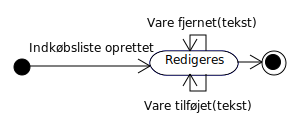
\includegraphics[scale=1]{billeder/foodl/thumbnails/indkoebsliste.png}
	\capt{Denne figur har til formål at give et overblik over systemets indkøbsliste.}
	\label{fig:overblik-indkoebsliste}
\end{figure}

Brugeren har mulighed for at tilføje varer i feltet ``tilføj til indkøbsliste'' og trykke på ``tilføj'' i bunden af siden. Der er mulighed for at slette alle varer fra indkøbslisten, ved at trykke på knappen ``slet alt'' i øverste højre hjørne af indkøbslisten, og ligeledes at slette enkelte varer, ved at trykke på de små gule krydser ud for alle varerne. Derudover er der implementeret en knap, til at udskrive indkøbslisten, som vi naturligvis kalder for ``udskriv''.

Hvis brugeren ikke er logget ind, vil de se i øverste højre hjørne af \figref{fig:overblik-indkoebsliste} (under sidehovedet) en boks, som informerer brugeren om, at man skal være logget ind for at systemet skal være i stand til at gemme indkøbslisten og favoritter. Oprettelse af bruger og indlogning bliver beskrevet nærmere i \secref{subsec:brug-opret}.

\subsection{Favoritliste}
\label{subsec:brug-favoritliste}

Når der bliver tilføjet en opskrift til en brugers favoritliste, så kan denne opskrift findes under ``favoritter'', som kan findes via sidehovedet i toppen af siden. Et eksempel af en kort opskriftsliste under favoritter kan ses på \figref{fig:overblik-favoritter}.

\begin{figure}[H]
	\centering
	\includegraphics[scale=1]{billeder/foodl/thumbnails/favoritter.png}
	\capt{Denne figur har til formål at give et overblik over systemets favoritside.}
	\label{fig:overblik-favoritter}
\end{figure}

En opskrift bliver tilføjet til favoritlisten ved at trykke på den hjerte-formede knap i øverste højre hjørne af en opskrift. Hvis en opskrift ikke er favoriseret, så er det hjerteformede område i knappen gråt. Når den bliver favoriseret, så bliver hjertet rødt, og dette kan ses i \figref{fig:overblik-favoritter}.

Idéen med favoritlisten er at give brugerne mulighed for at gemme opskrifter, de finder interessante og at de gerne vil bogmærke den til næste gang. De er meget nemmere at finde frem, når man kan finde dem under favoritlisten i stedet for at skulle udføre en ny søgning og prøve at finde den samme opskrift igen.

\subsection{Brugeroprettelse}
\label{subsec:brug-opret}

Alle har mulighed for at oprette en bruger på \Foodl{}. Hvis man har en bruger og logger ind på systemet, så kan man kan gemme sin indkøbsliste og listen over favoritter. Det er dog ikke obligatorisk at have en bruger for at kunne bruge systemet, da vi ikke ønsker at binde brugerne til at oprette noget som helst. Man kan bruge hele systemet, om man har en bruger eller ej.

Man opretter en bruger på samme side, hvor man logger ind på systemet. Dette er præsenteret i \figref{fig:overblik-brugeroprettelse}. Man navigerer til denne side ved at klikke på ``log ind / opret bruger'' i højre side af sidehovedet, som også er synlig på samme figur.

\begin{figure}[H]
	\centering
	\includegraphics[scale=0.4]{billeder/foodl/thumbnails/opretbrugeroglogind.png}
	\capt{Denne figur har til formål at give et overblik over systemets brugeroprettelsesside.}
	\label{fig:overblik-brugeroprettelse}
\end{figure}

Man skal bruge sin email og en adgangskode for at lave en bruger. Hvis man allerede har en bruger, så skal man blot logge ind med de rigtige oplysninger.

Når man er logget ind, så ændrer sidehovedet sig en smule. Figur \ref{fig:foodl-loggetind} viser, at der nu er mulighed for at gå ind i en menu, der hedder ``indstillinger'' og at logge ud igen. Man kan også se, at der pludselig er indlæst en liste af favoritter på 10 opskrifter fra tidligere et besøg.

\begin{figure}[H]
	\centering
	\includegraphics[scale=0.4]{billeder/foodl/header-login.png}
	\capt{Det ændrede sidehovede, når brugeren er logget ind.}
	\label{fig:foodl-loggetind}
\end{figure}

Hvis man ønsker at skifte sin adgangskode, så sker det ved at trykke på knappen ``indstillinger'' i sidehovedet.

\subsection{Generelt}
Som de fleste andre hjemmesider, så har vi også en ``om'' og en ``kontakt'' side, som kan tilgås fra nederste venstre hjørne af enhver underside af \Foodl{}. Derudover kan man rapportere en generel fejl ved siden, hvis man støder på sådan en. Figur \ref{fig:foodl-formaliteter} viser disse tre knapper.

\begin{figure}[H]
	\centering
	\includegraphics[scale=0.7]{billeder/foodl/formaliteter.jpg}
	\capt{I nederste venstre hjørne af systemet kan man rapportere en generel fejl, læse mere om systemet og kontakte udviklerne.}
	\label{fig:foodl-formaliteter}
\end{figure}

Under ``om foodl'' kan brugeren kort læse om dette projekt og om udviklerne bag systemet, altså denne gruppe.

\subsection{Designovervejelser}
\label{subsec:designovervejelser}

\todo{DEB!}